\documentclass[aspectratio=169]{beamer}

\usetheme{Boadilla}
\usefonttheme{professionalfonts}
\setbeamertemplate{navigation symbols}{}
\setbeamertemplate{itemize items}[circle]
\setbeamertemplate{enumerate items}[default]
\setbeamertemplate{headline}{}

\usepackage[utf8]{inputenc}
\usepackage[T1]{fontenc}
\usepackage{lmodern}
\usepackage{amsmath}
\usepackage{booktabs}
\usepackage{tabularx}
\usepackage{array}
\usepackage{hyperref}
\usepackage[strings]{underscore}
\usepackage{listings}
\usepackage{tikz}
\usetikzlibrary{arrows.meta,positioning,fit,calc,shapes.geometric}
\usepackage{xcolor}

\definecolor{courseblue}{HTML}{12355B}
\definecolor{coursegold}{HTML}{C98A2E}
\definecolor{courseice}{HTML}{EEF3F8}
\definecolor{coursegreen}{HTML}{2F6B4F}
\definecolor{coursegray}{HTML}{4B5563}
\definecolor{codebg}{HTML}{F7F9FC}
\definecolor{codecomment}{HTML}{5E6C84}
\definecolor{codestring}{HTML}{0B6E4F}

\setbeamercolor{palette primary}{bg=courseblue,fg=white}
\setbeamercolor{palette secondary}{bg=coursegold,fg=white}
\setbeamercolor{palette tertiary}{bg=courseblue,fg=white}
\setbeamercolor{palette quaternary}{bg=coursegold,fg=white}
\setbeamercolor{structure}{fg=courseblue}
\setbeamercolor{frametitle}{bg=courseice,fg=courseblue}
\setbeamercolor{title}{fg=courseblue}
\setbeamercolor{block title}{bg=courseblue,fg=white}
\setbeamercolor{block body}{bg=courseice,fg=black}
\setbeamercolor{normal text}{fg=black,bg=white}
\setbeamercolor{alerted text}{fg=coursegold}

\setbeamerfont{footline}{size=\scriptsize}

\setbeamertemplate{footline}{
  \leavevmode
  \hbox{
    \begin{beamercolorbox}[wd=.33\paperwidth,ht=2.8ex,dp=1.2ex,leftskip=0.8em]{palette primary}%
      University of Trieste
    \end{beamercolorbox}%
    \begin{beamercolorbox}[wd=.49\paperwidth,ht=2.8ex,dp=1.2ex,center]{palette tertiary}%
      \coursename{} \textbar{} \coursecode
    \end{beamercolorbox}%
    \begin{beamercolorbox}[wd=.18\paperwidth,ht=2.8ex,dp=1.2ex,rightskip=0.8em plus1fil]{palette secondary}%
      \insertframenumber{} / \inserttotalframenumber
    \end{beamercolorbox}%
  }
}

\hypersetup{
  colorlinks=true,
  linkcolor=courseblue,
  urlcolor=coursegreen
}

\lstdefinestyle{coursepython}{
  language=Python,
  basicstyle=\ttfamily\footnotesize,
  keywordstyle=\color{courseblue}\bfseries,
  commentstyle=\color{codecomment}\itshape,
  stringstyle=\color{codestring},
  showstringspaces=false,
  columns=fullflexible,
  keepspaces=true,
  frame=single,
  framerule=0.6pt,
  rulecolor=\color{courseblue},
  backgroundcolor=\color{codebg},
  xleftmargin=0.4em,
  xrightmargin=0.4em,
  aboveskip=0.4em,
  belowskip=0.2em
}

\newcommand{\coursename}{Data-driven Systems Engineering}
\newcommand{\coursecode}{440MI / 305SM}
\newcommand{\coursefooter}{}

\newcommand{\learninggoals}[1]{
  \begin{block}{Learning goals}
  #1
  \end{block}
}

\newcommand{\repoactivity}[1]{
  \begin{block}{Repo activity}
  #1
  \end{block}
}

\newcommand{\readinglist}[1]{
  \begin{block}{Papers and materials}
  {\footnotesize #1}
  \end{block}
}

\newcommand{\coursecontextframe}[5]{
  \begin{frame}{Course Map and Running Cases}
  \centering
  \begin{tikzpicture}[node distance=0.28cm]
  \node[flowbox, minimum width=1.45cm, minimum height=0.8cm] (problem) {\scriptsize Problem};
  \node[flowbox, minimum width=1.45cm, minimum height=0.8cm, right=of problem] (data) {\scriptsize Data};
  \node[flowbox, minimum width=1.45cm, minimum height=0.8cm, right=of data] (features) {\scriptsize Features};
  \node[flowbox, minimum width=1.45cm, minimum height=0.8cm, right=of features] (model) {\scriptsize Model};
  \node[flowbox, minimum width=1.45cm, minimum height=0.8cm, right=of model] (interface) {\scriptsize Interface};
  \node[flowbox, minimum width=1.45cm, minimum height=0.8cm, right=of interface] (delivery) {\scriptsize Delivery};
  \node[flowbox, minimum width=1.45cm, minimum height=0.8cm, right=of delivery] (monitor) {\scriptsize Monitor};
  \node[accentbox, minimum width=1.6cm, minimum height=0.8cm, right=of monitor] (evolution) {\scriptsize Evolution};
  \foreach \a/\b in {problem/data,data/features,features/model,model/interface,interface/delivery,delivery/monitor,monitor/evolution} {
    \draw[arrow] (\a) -- (\b);
  }
  \end{tikzpicture}

  \vspace{0.5em}
  \begin{block}{Today in the course}
  \textbf{Focus:} #1

  \textbf{Bridge:} #2
  \end{block}

  \begin{columns}[T]
  \column{0.48\textwidth}
  \begin{block}{Fraud case}
  {\footnotesize #3}
  \end{block}
  \column{0.48\textwidth}
  \begin{block}{Pasteurization case}
  {\footnotesize #4}
  \end{block}
  \end{columns}

  \vspace{0.3em}
  {\footnotesize \textbf{Course thread:} #5}
  \coursefooter
  \end{frame}
}

\newcommand{\classclosingframe}[4]{
  \begin{frame}{From This Class to the Next}
  \begin{block}{What stays with us}
  #1
  \end{block}

  \begin{columns}[T]
  \column{0.48\textwidth}
  \begin{block}{Project use}
  {\footnotesize #2}
  \end{block}
  \column{0.48\textwidth}
  \begin{block}{Next connection}
  {\footnotesize #3}
  \end{block}
  \end{columns}

  \vspace{0.3em}
  {\footnotesize \textbf{Course thread:} #4}
  \coursefooter
  \end{frame}
}

\tikzset{
  flowbox/.style={
    rounded corners=3pt,
    draw=courseblue,
    fill=courseice,
    very thick,
    minimum width=2.2cm,
    minimum height=0.9cm,
    align=center,
    font=\small
  },
  accentbox/.style={
    rounded corners=3pt,
    draw=coursegold,
    fill=coursegold!15,
    very thick,
    minimum width=2.2cm,
    minimum height=0.9cm,
    align=center,
    font=\small
  },
  arrow/.style={
    -{Latex[length=2.5mm,width=2mm]},
    thick,
    draw=courseblue
  }
}

% Visual layer on top of common.tex: tiles, icons, a progress-strip section divider, and a footer
% strip that defines the concepts appearing for the first time on each slide.
% Same look as the Class 20 deck. Load with:  \documentclass[aspectratio=169]{beamer}

\usetheme{Boadilla}
\usefonttheme{professionalfonts}
\setbeamertemplate{navigation symbols}{}
\setbeamertemplate{itemize items}[circle]
\setbeamertemplate{enumerate items}[default]
\setbeamertemplate{headline}{}

\usepackage[utf8]{inputenc}
\usepackage[T1]{fontenc}
\usepackage{lmodern}
\usepackage{amsmath}
\usepackage{booktabs}
\usepackage{tabularx}
\usepackage{array}
\usepackage{hyperref}
\usepackage[strings]{underscore}
\usepackage{listings}
\usepackage{tikz}
\usetikzlibrary{arrows.meta,positioning,fit,calc,shapes.geometric}
\usepackage{xcolor}

\definecolor{courseblue}{HTML}{12355B}
\definecolor{coursegold}{HTML}{C98A2E}
\definecolor{courseice}{HTML}{EEF3F8}
\definecolor{coursegreen}{HTML}{2F6B4F}
\definecolor{coursegray}{HTML}{4B5563}
\definecolor{codebg}{HTML}{F7F9FC}
\definecolor{codecomment}{HTML}{5E6C84}
\definecolor{codestring}{HTML}{0B6E4F}

\setbeamercolor{palette primary}{bg=courseblue,fg=white}
\setbeamercolor{palette secondary}{bg=coursegold,fg=white}
\setbeamercolor{palette tertiary}{bg=courseblue,fg=white}
\setbeamercolor{palette quaternary}{bg=coursegold,fg=white}
\setbeamercolor{structure}{fg=courseblue}
\setbeamercolor{frametitle}{bg=courseice,fg=courseblue}
\setbeamercolor{title}{fg=courseblue}
\setbeamercolor{block title}{bg=courseblue,fg=white}
\setbeamercolor{block body}{bg=courseice,fg=black}
\setbeamercolor{normal text}{fg=black,bg=white}
\setbeamercolor{alerted text}{fg=coursegold}

\setbeamerfont{footline}{size=\scriptsize}

\setbeamertemplate{footline}{
  \leavevmode
  \hbox{
    \begin{beamercolorbox}[wd=.33\paperwidth,ht=2.8ex,dp=1.2ex,leftskip=0.8em]{palette primary}%
      University of Trieste
    \end{beamercolorbox}%
    \begin{beamercolorbox}[wd=.49\paperwidth,ht=2.8ex,dp=1.2ex,center]{palette tertiary}%
      \coursename{} \textbar{} \coursecode
    \end{beamercolorbox}%
    \begin{beamercolorbox}[wd=.18\paperwidth,ht=2.8ex,dp=1.2ex,rightskip=0.8em plus1fil]{palette secondary}%
      \insertframenumber{} / \inserttotalframenumber
    \end{beamercolorbox}%
  }
}

\hypersetup{
  colorlinks=true,
  linkcolor=courseblue,
  urlcolor=coursegreen
}

\lstdefinestyle{coursepython}{
  language=Python,
  basicstyle=\ttfamily\footnotesize,
  keywordstyle=\color{courseblue}\bfseries,
  commentstyle=\color{codecomment}\itshape,
  stringstyle=\color{codestring},
  showstringspaces=false,
  columns=fullflexible,
  keepspaces=true,
  frame=single,
  framerule=0.6pt,
  rulecolor=\color{courseblue},
  backgroundcolor=\color{codebg},
  xleftmargin=0.4em,
  xrightmargin=0.4em,
  aboveskip=0.4em,
  belowskip=0.2em
}

\newcommand{\coursename}{Data-driven Systems Engineering}
\newcommand{\coursecode}{440MI / 305SM}
\newcommand{\coursefooter}{}

\newcommand{\learninggoals}[1]{
  \begin{block}{Learning goals}
  #1
  \end{block}
}

\newcommand{\repoactivity}[1]{
  \begin{block}{Repo activity}
  #1
  \end{block}
}

\newcommand{\readinglist}[1]{
  \begin{block}{Papers and materials}
  {\footnotesize #1}
  \end{block}
}

\newcommand{\coursecontextframe}[5]{
  \begin{frame}{Course Map and Running Cases}
  \centering
  \begin{tikzpicture}[node distance=0.28cm]
  \node[flowbox, minimum width=1.45cm, minimum height=0.8cm] (problem) {\scriptsize Problem};
  \node[flowbox, minimum width=1.45cm, minimum height=0.8cm, right=of problem] (data) {\scriptsize Data};
  \node[flowbox, minimum width=1.45cm, minimum height=0.8cm, right=of data] (features) {\scriptsize Features};
  \node[flowbox, minimum width=1.45cm, minimum height=0.8cm, right=of features] (model) {\scriptsize Model};
  \node[flowbox, minimum width=1.45cm, minimum height=0.8cm, right=of model] (interface) {\scriptsize Interface};
  \node[flowbox, minimum width=1.45cm, minimum height=0.8cm, right=of interface] (delivery) {\scriptsize Delivery};
  \node[flowbox, minimum width=1.45cm, minimum height=0.8cm, right=of delivery] (monitor) {\scriptsize Monitor};
  \node[accentbox, minimum width=1.6cm, minimum height=0.8cm, right=of monitor] (evolution) {\scriptsize Evolution};
  \foreach \a/\b in {problem/data,data/features,features/model,model/interface,interface/delivery,delivery/monitor,monitor/evolution} {
    \draw[arrow] (\a) -- (\b);
  }
  \end{tikzpicture}

  \vspace{0.5em}
  \begin{block}{Today in the course}
  \textbf{Focus:} #1

  \textbf{Bridge:} #2
  \end{block}

  \begin{columns}[T]
  \column{0.48\textwidth}
  \begin{block}{Fraud case}
  {\footnotesize #3}
  \end{block}
  \column{0.48\textwidth}
  \begin{block}{Pasteurization case}
  {\footnotesize #4}
  \end{block}
  \end{columns}

  \vspace{0.3em}
  {\footnotesize \textbf{Course thread:} #5}
  \coursefooter
  \end{frame}
}

\newcommand{\classclosingframe}[4]{
  \begin{frame}{From This Class to the Next}
  \begin{block}{What stays with us}
  #1
  \end{block}

  \begin{columns}[T]
  \column{0.48\textwidth}
  \begin{block}{Project use}
  {\footnotesize #2}
  \end{block}
  \column{0.48\textwidth}
  \begin{block}{Next connection}
  {\footnotesize #3}
  \end{block}
  \end{columns}

  \vspace{0.3em}
  {\footnotesize \textbf{Course thread:} #4}
  \coursefooter
  \end{frame}
}

\tikzset{
  flowbox/.style={
    rounded corners=3pt,
    draw=courseblue,
    fill=courseice,
    very thick,
    minimum width=2.2cm,
    minimum height=0.9cm,
    align=center,
    font=\small
  },
  accentbox/.style={
    rounded corners=3pt,
    draw=coursegold,
    fill=coursegold!15,
    very thick,
    minimum width=2.2cm,
    minimum height=0.9cm,
    align=center,
    font=\small
  },
  arrow/.style={
    -{Latex[length=2.5mm,width=2mm]},
    thick,
    draw=courseblue
  }
}
  % Visual layer on top of common.tex: tiles, icons, a progress-strip section divider, and a footer
% strip that defines the concepts appearing for the first time on each slide.
% Same look as the Class 20 deck. Load with:  \documentclass[aspectratio=169]{beamer}

\usetheme{Boadilla}
\usefonttheme{professionalfonts}
\setbeamertemplate{navigation symbols}{}
\setbeamertemplate{itemize items}[circle]
\setbeamertemplate{enumerate items}[default]
\setbeamertemplate{headline}{}

\usepackage[utf8]{inputenc}
\usepackage[T1]{fontenc}
\usepackage{lmodern}
\usepackage{amsmath}
\usepackage{booktabs}
\usepackage{tabularx}
\usepackage{array}
\usepackage{hyperref}
\usepackage[strings]{underscore}
\usepackage{listings}
\usepackage{tikz}
\usetikzlibrary{arrows.meta,positioning,fit,calc,shapes.geometric}
\usepackage{xcolor}

\definecolor{courseblue}{HTML}{12355B}
\definecolor{coursegold}{HTML}{C98A2E}
\definecolor{courseice}{HTML}{EEF3F8}
\definecolor{coursegreen}{HTML}{2F6B4F}
\definecolor{coursegray}{HTML}{4B5563}
\definecolor{codebg}{HTML}{F7F9FC}
\definecolor{codecomment}{HTML}{5E6C84}
\definecolor{codestring}{HTML}{0B6E4F}

\setbeamercolor{palette primary}{bg=courseblue,fg=white}
\setbeamercolor{palette secondary}{bg=coursegold,fg=white}
\setbeamercolor{palette tertiary}{bg=courseblue,fg=white}
\setbeamercolor{palette quaternary}{bg=coursegold,fg=white}
\setbeamercolor{structure}{fg=courseblue}
\setbeamercolor{frametitle}{bg=courseice,fg=courseblue}
\setbeamercolor{title}{fg=courseblue}
\setbeamercolor{block title}{bg=courseblue,fg=white}
\setbeamercolor{block body}{bg=courseice,fg=black}
\setbeamercolor{normal text}{fg=black,bg=white}
\setbeamercolor{alerted text}{fg=coursegold}

\setbeamerfont{footline}{size=\scriptsize}

\setbeamertemplate{footline}{
  \leavevmode
  \hbox{
    \begin{beamercolorbox}[wd=.33\paperwidth,ht=2.8ex,dp=1.2ex,leftskip=0.8em]{palette primary}%
      University of Trieste
    \end{beamercolorbox}%
    \begin{beamercolorbox}[wd=.49\paperwidth,ht=2.8ex,dp=1.2ex,center]{palette tertiary}%
      \coursename{} \textbar{} \coursecode
    \end{beamercolorbox}%
    \begin{beamercolorbox}[wd=.18\paperwidth,ht=2.8ex,dp=1.2ex,rightskip=0.8em plus1fil]{palette secondary}%
      \insertframenumber{} / \inserttotalframenumber
    \end{beamercolorbox}%
  }
}

\hypersetup{
  colorlinks=true,
  linkcolor=courseblue,
  urlcolor=coursegreen
}

\lstdefinestyle{coursepython}{
  language=Python,
  basicstyle=\ttfamily\footnotesize,
  keywordstyle=\color{courseblue}\bfseries,
  commentstyle=\color{codecomment}\itshape,
  stringstyle=\color{codestring},
  showstringspaces=false,
  columns=fullflexible,
  keepspaces=true,
  frame=single,
  framerule=0.6pt,
  rulecolor=\color{courseblue},
  backgroundcolor=\color{codebg},
  xleftmargin=0.4em,
  xrightmargin=0.4em,
  aboveskip=0.4em,
  belowskip=0.2em
}

\newcommand{\coursename}{Data-driven Systems Engineering}
\newcommand{\coursecode}{440MI / 305SM}
\newcommand{\coursefooter}{}

\newcommand{\learninggoals}[1]{
  \begin{block}{Learning goals}
  #1
  \end{block}
}

\newcommand{\repoactivity}[1]{
  \begin{block}{Repo activity}
  #1
  \end{block}
}

\newcommand{\readinglist}[1]{
  \begin{block}{Papers and materials}
  {\footnotesize #1}
  \end{block}
}

\newcommand{\coursecontextframe}[5]{
  \begin{frame}{Course Map and Running Cases}
  \centering
  \begin{tikzpicture}[node distance=0.28cm]
  \node[flowbox, minimum width=1.45cm, minimum height=0.8cm] (problem) {\scriptsize Problem};
  \node[flowbox, minimum width=1.45cm, minimum height=0.8cm, right=of problem] (data) {\scriptsize Data};
  \node[flowbox, minimum width=1.45cm, minimum height=0.8cm, right=of data] (features) {\scriptsize Features};
  \node[flowbox, minimum width=1.45cm, minimum height=0.8cm, right=of features] (model) {\scriptsize Model};
  \node[flowbox, minimum width=1.45cm, minimum height=0.8cm, right=of model] (interface) {\scriptsize Interface};
  \node[flowbox, minimum width=1.45cm, minimum height=0.8cm, right=of interface] (delivery) {\scriptsize Delivery};
  \node[flowbox, minimum width=1.45cm, minimum height=0.8cm, right=of delivery] (monitor) {\scriptsize Monitor};
  \node[accentbox, minimum width=1.6cm, minimum height=0.8cm, right=of monitor] (evolution) {\scriptsize Evolution};
  \foreach \a/\b in {problem/data,data/features,features/model,model/interface,interface/delivery,delivery/monitor,monitor/evolution} {
    \draw[arrow] (\a) -- (\b);
  }
  \end{tikzpicture}

  \vspace{0.5em}
  \begin{block}{Today in the course}
  \textbf{Focus:} #1

  \textbf{Bridge:} #2
  \end{block}

  \begin{columns}[T]
  \column{0.48\textwidth}
  \begin{block}{Fraud case}
  {\footnotesize #3}
  \end{block}
  \column{0.48\textwidth}
  \begin{block}{Pasteurization case}
  {\footnotesize #4}
  \end{block}
  \end{columns}

  \vspace{0.3em}
  {\footnotesize \textbf{Course thread:} #5}
  \coursefooter
  \end{frame}
}

\newcommand{\classclosingframe}[4]{
  \begin{frame}{From This Class to the Next}
  \begin{block}{What stays with us}
  #1
  \end{block}

  \begin{columns}[T]
  \column{0.48\textwidth}
  \begin{block}{Project use}
  {\footnotesize #2}
  \end{block}
  \column{0.48\textwidth}
  \begin{block}{Next connection}
  {\footnotesize #3}
  \end{block}
  \end{columns}

  \vspace{0.3em}
  {\footnotesize \textbf{Course thread:} #4}
  \coursefooter
  \end{frame}
}

\tikzset{
  flowbox/.style={
    rounded corners=3pt,
    draw=courseblue,
    fill=courseice,
    very thick,
    minimum width=2.2cm,
    minimum height=0.9cm,
    align=center,
    font=\small
  },
  accentbox/.style={
    rounded corners=3pt,
    draw=coursegold,
    fill=coursegold!15,
    very thick,
    minimum width=2.2cm,
    minimum height=0.9cm,
    align=center,
    font=\small
  },
  arrow/.style={
    -{Latex[length=2.5mm,width=2mm]},
    thick,
    draw=courseblue
  }
}
  % Visual layer on top of common.tex: tiles, icons, a progress-strip section divider, and a footer
% strip that defines the concepts appearing for the first time on each slide.
% Same look as the Class 20 deck. Load with:  \input{common}  \input{common_visual}
%
% Before the first \sectiondivider, a deck must define
%   \sectioncount   the number of sections, e.g. 4
%   \sectionlabels  a \foreach list of number/label pairs, e.g. 1/Need,2/Testable,3/Manage,4/Practice
% Icons come from the fontawesome5 package (Font Awesome 5 Free), e.g. \faIcon{robot}.

\usepackage{colortbl}
\usepackage{fontawesome5}
\usetikzlibrary{backgrounds}

% Slides read better without automatic hyphenation.
\hyphenpenalty=10000
\exhyphenpenalty=10000

\definecolor{coursered}{HTML}{A23B2A}
\newcommand{\goldink}{\color{coursegold!65!black}}

\tikzset{
  tile/.style={rounded corners=4pt, fill=courseice, draw=none, align=center, font=\footnotesize, inner sep=5pt},
  tileblue/.style={tile, fill=white, draw=courseblue!55, thick},
  tilegold/.style={tile, fill=coursegold!14, draw=coursegold, thick},
  tilegreen/.style={tile, fill=coursegreen!10, draw=coursegreen!70, thick},
  tilered/.style={tile, fill=coursered!8, draw=coursered!70, thick},
  tilegray/.style={tile, fill=white, draw=coursegray!55, thick, dashed},
  tag/.style={rounded corners=2pt, fill=coursegold, text=white, font=\bfseries\tiny, inner sep=2.5pt},
  chip/.style={rounded corners=3pt, fill=courseblue, text=white, font=\footnotesize\bfseries, align=center, inner sep=4pt},
  note/.style={font=\scriptsize, text=coursegray, align=left},
  arrowgold/.style={-{Latex[length=2.5mm,width=2mm]}, thick, draw=coursegold},
  arrowred/.style={-{Latex[length=2.5mm,width=2mm]}, thick, draw=coursered},
  arrowgreen/.style={-{Latex[length=2.5mm,width=2mm]}, thick, draw=coursegreen},
  arrowgray/.style={-{Latex[length=2mm,width=1.6mm]}, thick, draw=coursegray!70},
}

% A round icon badge, drawn inside a tikzpicture: x y colour icon
\newcommand{\badge}[4]{%
  \node[circle, fill=#3, text=white, minimum size=0.85cm, inner sep=0pt] at (#1,#2) {\large\faIcon{#4}};
}

% Inline tags for the kind of requirement.
\newcommand{\Ftag}{\colorbox{courseblue}{\color{white}\bfseries\scriptsize\ \ F\ \ }}
\newcommand{\NFtag}{\colorbox{coursegold}{\color{white}\bfseries\scriptsize\ NF\ }}
\newcommand{\Dtag}{\colorbox{coursegreen}{\color{white}\bfseries\scriptsize\ \ D\ \ }}
\newcommand{\MLtag}{\colorbox{coursered}{\color{white}\bfseries\scriptsize\ ML\ }}

% Footer: a strip with the concepts that appear for the first time on the slide, above the
% usual bar. The bar total counts only the main lecture; a backup slide is numbered separately.
\makeatletter
\def\conceptstext{}
\def\currentsectionname{}
\setbeamercolor{conceptbar}{bg=coursegold!12,fg=black}
\newcommand{\cterm}[2]{{\bfseries\color{courseblue}#1:}\ #2\hspace{0.8em}}
\newcommand{\newtag}{\colorbox{coursegold}{\color{white}\bfseries\tiny\ NEW\ }\hspace{0.6em}}
\setbeamertemplate{footline}{
  \leavevmode
  \vbox{%
    \ifx\conceptstext\empty\else
      \hbox{\color{coursegold}\rule{\paperwidth}{0.8pt}}%
      \hbox{\begin{beamercolorbox}[wd=\paperwidth,leftskip=0.5cm,rightskip=0.5cm,sep=3pt]{conceptbar}\scriptsize\newtag\conceptstext\end{beamercolorbox}}%
    \fi
    \hbox{%
      \begin{beamercolorbox}[wd=.33\paperwidth,ht=2.8ex,dp=1.2ex,leftskip=0.8em]{palette primary}%
        \ifbeamer@inappendix Backup\else\ifnum\value{section}>0 \arabic{section}\ \textbar\ \currentsectionname\else University of Trieste\fi\fi
      \end{beamercolorbox}%
      \begin{beamercolorbox}[wd=.49\paperwidth,ht=2.8ex,dp=1.2ex,center]{palette tertiary}%
        \coursename{} \textbar{} \coursecode
      \end{beamercolorbox}%
      \begin{beamercolorbox}[wd=.18\paperwidth,ht=2.8ex,dp=1.2ex,right,rightskip=0.8em]{palette secondary}%
        \ifbeamer@inappendix Backup \insertframenumberinappendix\else\insertframenumber{} / \insertmainframenumber\fi
      \end{beamercolorbox}%
    }}}
\makeatother
\newenvironment{cframe}[2]{\gdef\conceptstext{#2}\begin{frame}{#1}}{\end{frame}\gdef\conceptstext{}}

% Section divider: progress strip, recap of the previous part, and the roadmap of the next one.
% Arguments: number, title, icon, previously, items.
\newcommand{\sectiondivider}[5]{%
  \section{#2}\gdef\currentsectionname{#2}
  \begin{frame}
  \centering
  \begin{tikzpicture}
  \pgfmathsetmacro{\chipw}{13.6/\sectioncount}
  \foreach \i/\lab in \sectionlabels {
    \ifnum\i<#1 \def\chipfill{courseblue!22}\def\chiptext{courseblue}\else
    \ifnum\i=#1 \def\chipfill{courseblue}\def\chiptext{white}\else
    \def\chipfill{courseice}\def\chiptext{coursegray}\fi\fi
    \node[rounded corners=3pt, minimum width={(\chipw-0.1)*1cm}, minimum height=0.6cm, font=\scriptsize\bfseries, fill=\chipfill, text=\chiptext] at ({\chipw/2+(\i-1)*\chipw},0) {\i\ \lab};
  }
  \node[circle, fill=courseblue, text=white, font=\Huge\bfseries, minimum size=1.7cm, inner sep=0] at (1.0,-1.7) {#1};
  \node[anchor=west, font=\huge\bfseries, text=courseblue, text width=8.8cm, align=left] at (2.2,-1.7) {#2};
  \node[circle, fill=coursegold!16, draw=coursegold, thick, text=coursegold!75!black, font=\fontsize{26}{26}\selectfont, minimum size=1.9cm, inner sep=0] at (12.6,-1.7) {\faIcon{#3}};
  \ifx\relax#4\relax\else
    \node[anchor=north west, font=\small\itshape, text=coursegray, text width=13.2cm, align=left] at (0.1,-2.95) {Previously: #4};
  \fi
  \node[anchor=north west, font=\footnotesize\bfseries, text=coursegold!65!black] at (0.1,-3.95) {IN THIS PART};
  \node[anchor=north west, font=\small, text width=13.2cm, align=left] at (0.1,-4.35) {#5};
  \end{tikzpicture}
  \end{frame}
}

%
% Before the first \sectiondivider, a deck must define
%   \sectioncount   the number of sections, e.g. 4
%   \sectionlabels  a \foreach list of number/label pairs, e.g. 1/Need,2/Testable,3/Manage,4/Practice
% Icons come from the fontawesome5 package (Font Awesome 5 Free), e.g. \faIcon{robot}.

\usepackage{colortbl}
\usepackage{fontawesome5}
\usetikzlibrary{backgrounds}

% Slides read better without automatic hyphenation.
\hyphenpenalty=10000
\exhyphenpenalty=10000

\definecolor{coursered}{HTML}{A23B2A}
\newcommand{\goldink}{\color{coursegold!65!black}}

\tikzset{
  tile/.style={rounded corners=4pt, fill=courseice, draw=none, align=center, font=\footnotesize, inner sep=5pt},
  tileblue/.style={tile, fill=white, draw=courseblue!55, thick},
  tilegold/.style={tile, fill=coursegold!14, draw=coursegold, thick},
  tilegreen/.style={tile, fill=coursegreen!10, draw=coursegreen!70, thick},
  tilered/.style={tile, fill=coursered!8, draw=coursered!70, thick},
  tilegray/.style={tile, fill=white, draw=coursegray!55, thick, dashed},
  tag/.style={rounded corners=2pt, fill=coursegold, text=white, font=\bfseries\tiny, inner sep=2.5pt},
  chip/.style={rounded corners=3pt, fill=courseblue, text=white, font=\footnotesize\bfseries, align=center, inner sep=4pt},
  note/.style={font=\scriptsize, text=coursegray, align=left},
  arrowgold/.style={-{Latex[length=2.5mm,width=2mm]}, thick, draw=coursegold},
  arrowred/.style={-{Latex[length=2.5mm,width=2mm]}, thick, draw=coursered},
  arrowgreen/.style={-{Latex[length=2.5mm,width=2mm]}, thick, draw=coursegreen},
  arrowgray/.style={-{Latex[length=2mm,width=1.6mm]}, thick, draw=coursegray!70},
}

% A round icon badge, drawn inside a tikzpicture: x y colour icon
\newcommand{\badge}[4]{%
  \node[circle, fill=#3, text=white, minimum size=0.85cm, inner sep=0pt] at (#1,#2) {\large\faIcon{#4}};
}

% Inline tags for the kind of requirement.
\newcommand{\Ftag}{\colorbox{courseblue}{\color{white}\bfseries\scriptsize\ \ F\ \ }}
\newcommand{\NFtag}{\colorbox{coursegold}{\color{white}\bfseries\scriptsize\ NF\ }}
\newcommand{\Dtag}{\colorbox{coursegreen}{\color{white}\bfseries\scriptsize\ \ D\ \ }}
\newcommand{\MLtag}{\colorbox{coursered}{\color{white}\bfseries\scriptsize\ ML\ }}

% Footer: a strip with the concepts that appear for the first time on the slide, above the
% usual bar. The bar total counts only the main lecture; a backup slide is numbered separately.
\makeatletter
\def\conceptstext{}
\def\currentsectionname{}
\setbeamercolor{conceptbar}{bg=coursegold!12,fg=black}
\newcommand{\cterm}[2]{{\bfseries\color{courseblue}#1:}\ #2\hspace{0.8em}}
\newcommand{\newtag}{\colorbox{coursegold}{\color{white}\bfseries\tiny\ NEW\ }\hspace{0.6em}}
\setbeamertemplate{footline}{
  \leavevmode
  \vbox{%
    \ifx\conceptstext\empty\else
      \hbox{\color{coursegold}\rule{\paperwidth}{0.8pt}}%
      \hbox{\begin{beamercolorbox}[wd=\paperwidth,leftskip=0.5cm,rightskip=0.5cm,sep=3pt]{conceptbar}\scriptsize\newtag\conceptstext\end{beamercolorbox}}%
    \fi
    \hbox{%
      \begin{beamercolorbox}[wd=.33\paperwidth,ht=2.8ex,dp=1.2ex,leftskip=0.8em]{palette primary}%
        \ifbeamer@inappendix Backup\else\ifnum\value{section}>0 \arabic{section}\ \textbar\ \currentsectionname\else University of Trieste\fi\fi
      \end{beamercolorbox}%
      \begin{beamercolorbox}[wd=.49\paperwidth,ht=2.8ex,dp=1.2ex,center]{palette tertiary}%
        \coursename{} \textbar{} \coursecode
      \end{beamercolorbox}%
      \begin{beamercolorbox}[wd=.18\paperwidth,ht=2.8ex,dp=1.2ex,right,rightskip=0.8em]{palette secondary}%
        \ifbeamer@inappendix Backup \insertframenumberinappendix\else\insertframenumber{} / \insertmainframenumber\fi
      \end{beamercolorbox}%
    }}}
\makeatother
\newenvironment{cframe}[2]{\gdef\conceptstext{#2}\begin{frame}{#1}}{\end{frame}\gdef\conceptstext{}}

% Section divider: progress strip, recap of the previous part, and the roadmap of the next one.
% Arguments: number, title, icon, previously, items.
\newcommand{\sectiondivider}[5]{%
  \section{#2}\gdef\currentsectionname{#2}
  \begin{frame}
  \centering
  \begin{tikzpicture}
  \pgfmathsetmacro{\chipw}{13.6/\sectioncount}
  \foreach \i/\lab in \sectionlabels {
    \ifnum\i<#1 \def\chipfill{courseblue!22}\def\chiptext{courseblue}\else
    \ifnum\i=#1 \def\chipfill{courseblue}\def\chiptext{white}\else
    \def\chipfill{courseice}\def\chiptext{coursegray}\fi\fi
    \node[rounded corners=3pt, minimum width={(\chipw-0.1)*1cm}, minimum height=0.6cm, font=\scriptsize\bfseries, fill=\chipfill, text=\chiptext] at ({\chipw/2+(\i-1)*\chipw},0) {\i\ \lab};
  }
  \node[circle, fill=courseblue, text=white, font=\Huge\bfseries, minimum size=1.7cm, inner sep=0] at (1.0,-1.7) {#1};
  \node[anchor=west, font=\huge\bfseries, text=courseblue, text width=8.8cm, align=left] at (2.2,-1.7) {#2};
  \node[circle, fill=coursegold!16, draw=coursegold, thick, text=coursegold!75!black, font=\fontsize{26}{26}\selectfont, minimum size=1.9cm, inner sep=0] at (12.6,-1.7) {\faIcon{#3}};
  \ifx\relax#4\relax\else
    \node[anchor=north west, font=\small\itshape, text=coursegray, text width=13.2cm, align=left] at (0.1,-2.95) {Previously: #4};
  \fi
  \node[anchor=north west, font=\footnotesize\bfseries, text=coursegold!65!black] at (0.1,-3.95) {IN THIS PART};
  \node[anchor=north west, font=\small, text width=13.2cm, align=left] at (0.1,-4.35) {#5};
  \end{tikzpicture}
  \end{frame}
}

%
% Before the first \sectiondivider, a deck must define
%   \sectioncount   the number of sections, e.g. 4
%   \sectionlabels  a \foreach list of number/label pairs, e.g. 1/Need,2/Testable,3/Manage,4/Practice
% Icons come from the fontawesome5 package (Font Awesome 5 Free), e.g. \faIcon{robot}.

\usepackage{colortbl}
\usepackage{fontawesome5}
\usetikzlibrary{backgrounds}

% Slides read better without automatic hyphenation.
\hyphenpenalty=10000
\exhyphenpenalty=10000

\definecolor{coursered}{HTML}{A23B2A}
\newcommand{\goldink}{\color{coursegold!65!black}}

\tikzset{
  tile/.style={rounded corners=4pt, fill=courseice, draw=none, align=center, font=\footnotesize, inner sep=5pt},
  tileblue/.style={tile, fill=white, draw=courseblue!55, thick},
  tilegold/.style={tile, fill=coursegold!14, draw=coursegold, thick},
  tilegreen/.style={tile, fill=coursegreen!10, draw=coursegreen!70, thick},
  tilered/.style={tile, fill=coursered!8, draw=coursered!70, thick},
  tilegray/.style={tile, fill=white, draw=coursegray!55, thick, dashed},
  tag/.style={rounded corners=2pt, fill=coursegold, text=white, font=\bfseries\tiny, inner sep=2.5pt},
  chip/.style={rounded corners=3pt, fill=courseblue, text=white, font=\footnotesize\bfseries, align=center, inner sep=4pt},
  note/.style={font=\scriptsize, text=coursegray, align=left},
  arrowgold/.style={-{Latex[length=2.5mm,width=2mm]}, thick, draw=coursegold},
  arrowred/.style={-{Latex[length=2.5mm,width=2mm]}, thick, draw=coursered},
  arrowgreen/.style={-{Latex[length=2.5mm,width=2mm]}, thick, draw=coursegreen},
  arrowgray/.style={-{Latex[length=2mm,width=1.6mm]}, thick, draw=coursegray!70},
}

% A round icon badge, drawn inside a tikzpicture: x y colour icon
\newcommand{\badge}[4]{%
  \node[circle, fill=#3, text=white, minimum size=0.85cm, inner sep=0pt] at (#1,#2) {\large\faIcon{#4}};
}

% Inline tags for the kind of requirement.
\newcommand{\Ftag}{\colorbox{courseblue}{\color{white}\bfseries\scriptsize\ \ F\ \ }}
\newcommand{\NFtag}{\colorbox{coursegold}{\color{white}\bfseries\scriptsize\ NF\ }}
\newcommand{\Dtag}{\colorbox{coursegreen}{\color{white}\bfseries\scriptsize\ \ D\ \ }}
\newcommand{\MLtag}{\colorbox{coursered}{\color{white}\bfseries\scriptsize\ ML\ }}

% Footer: a strip with the concepts that appear for the first time on the slide, above the
% usual bar. The bar total counts only the main lecture; a backup slide is numbered separately.
\makeatletter
\def\conceptstext{}
\def\currentsectionname{}
\setbeamercolor{conceptbar}{bg=coursegold!12,fg=black}
\newcommand{\cterm}[2]{{\bfseries\color{courseblue}#1:}\ #2\hspace{0.8em}}
\newcommand{\newtag}{\colorbox{coursegold}{\color{white}\bfseries\tiny\ NEW\ }\hspace{0.6em}}
\setbeamertemplate{footline}{
  \leavevmode
  \vbox{%
    \ifx\conceptstext\empty\else
      \hbox{\color{coursegold}\rule{\paperwidth}{0.8pt}}%
      \hbox{\begin{beamercolorbox}[wd=\paperwidth,leftskip=0.5cm,rightskip=0.5cm,sep=3pt]{conceptbar}\scriptsize\newtag\conceptstext\end{beamercolorbox}}%
    \fi
    \hbox{%
      \begin{beamercolorbox}[wd=.33\paperwidth,ht=2.8ex,dp=1.2ex,leftskip=0.8em]{palette primary}%
        \ifbeamer@inappendix Backup\else\ifnum\value{section}>0 \arabic{section}\ \textbar\ \currentsectionname\else University of Trieste\fi\fi
      \end{beamercolorbox}%
      \begin{beamercolorbox}[wd=.49\paperwidth,ht=2.8ex,dp=1.2ex,center]{palette tertiary}%
        \coursename{} \textbar{} \coursecode
      \end{beamercolorbox}%
      \begin{beamercolorbox}[wd=.18\paperwidth,ht=2.8ex,dp=1.2ex,right,rightskip=0.8em]{palette secondary}%
        \ifbeamer@inappendix Backup \insertframenumberinappendix\else\insertframenumber{} / \insertmainframenumber\fi
      \end{beamercolorbox}%
    }}}
\makeatother
\newenvironment{cframe}[2]{\gdef\conceptstext{#2}\begin{frame}{#1}}{\end{frame}\gdef\conceptstext{}}

% Section divider: progress strip, recap of the previous part, and the roadmap of the next one.
% Arguments: number, title, icon, previously, items.
\newcommand{\sectiondivider}[5]{%
  \section{#2}\gdef\currentsectionname{#2}
  \begin{frame}
  \centering
  \begin{tikzpicture}
  \pgfmathsetmacro{\chipw}{13.6/\sectioncount}
  \foreach \i/\lab in \sectionlabels {
    \ifnum\i<#1 \def\chipfill{courseblue!22}\def\chiptext{courseblue}\else
    \ifnum\i=#1 \def\chipfill{courseblue}\def\chiptext{white}\else
    \def\chipfill{courseice}\def\chiptext{coursegray}\fi\fi
    \node[rounded corners=3pt, minimum width={(\chipw-0.1)*1cm}, minimum height=0.6cm, font=\scriptsize\bfseries, fill=\chipfill, text=\chiptext] at ({\chipw/2+(\i-1)*\chipw},0) {\i\ \lab};
  }
  \node[circle, fill=courseblue, text=white, font=\Huge\bfseries, minimum size=1.7cm, inner sep=0] at (1.0,-1.7) {#1};
  \node[anchor=west, font=\huge\bfseries, text=courseblue, text width=8.8cm, align=left] at (2.2,-1.7) {#2};
  \node[circle, fill=coursegold!16, draw=coursegold, thick, text=coursegold!75!black, font=\fontsize{26}{26}\selectfont, minimum size=1.9cm, inner sep=0] at (12.6,-1.7) {\faIcon{#3}};
  \ifx\relax#4\relax\else
    \node[anchor=north west, font=\small\itshape, text=coursegray, text width=13.2cm, align=left] at (0.1,-2.95) {Previously: #4};
  \fi
  \node[anchor=north west, font=\footnotesize\bfseries, text=coursegold!65!black] at (0.1,-3.95) {IN THIS PART};
  \node[anchor=north west, font=\small, text width=13.2cm, align=left] at (0.1,-4.35) {#5};
  \end{tikzpicture}
  \end{frame}
}


% Three parts; the progress strip on each divider uses these labels.
\newcommand{\sectioncount}{3}
\newcommand{\sectionlabels}{1/Specify,2/Validate,3/Evolve}

\title{Class 28: Pasteurization Monitoring Challenge, Session 2}
\author{\coursename}
\date{}

\definecolor{stickyyellow}{HTML}{FBE8A6}
\definecolor{stickygreen}{HTML}{CFE6D6}
\definecolor{stickyblue}{HTML}{CFE0F1}

% ------------------------------------------------------------------ helpers
% A gold strip with the idea to remember: y text
\newcommand{\keyidea}[2]{%
  \node[tilegold, anchor=north west, minimum width=13.4cm, minimum height=0.8cm, text width=12.6cm, align=left, font=\footnotesize] at (0,#1) {{\bfseries\goldink\faIcon{lightbulb}\ Key idea.}\ #2};
}
% A sticky note: x y colour rotation text
\newcommand{\sticky}[5]{%
  \node[fill=#3, draw=#3!55!black, line width=0.3pt, minimum width=1.55cm, minimum height=0.46cm, text width=1.4cm, align=center, font=\tiny, text=black, inner sep=2pt, rotate=#4] at (#1,#2) {#5};
}
% A numbered step card (2.55 x 3.7 cm): x number icon colour title text
\newcommand{\stepcard}[6]{%
  \node[tile, fill=white, draw=#4, thick, anchor=north west, minimum width=2.55cm, minimum height=3.7cm] at (#1,0) {};
  \node[circle, fill=#4, text=white, minimum size=0.55cm, inner sep=0, font=\small\bfseries] at (#1+0.42,-0.42) {#2};
  \node[text=#4!70, font=\Large] at (#1+2.1,-0.42) {\faIcon{#3}};
  \node[anchor=north west, text width=2.2cm, align=left, font=\footnotesize\bfseries, text=courseblue, inner sep=0pt] at (#1+0.2,-0.88) {#5};
  \node[anchor=north west, text width=2.2cm, align=left, font=\scriptsize, inner sep=0pt] at (#1+0.2,-1.7) {#6};
}

% One example requirement (13.4 x 1.0 cm): y id source requirement check colour
\newcommand{\reqrow}[6]{%
  \node[chip, fill=#6, anchor=north west, minimum width=1.65cm, minimum height=1.08cm, font=\scriptsize\bfseries] at (0,#1) {#2\\{\tiny #3}};
  \node[tile, fill=white, draw=#6!70, thick, anchor=north west, minimum width=6.7cm, minimum height=1.08cm, text width=6.35cm, align=left, font=\scriptsize, inner sep=3pt] at (1.8,#1) {#4};
  \node[tile, fill=courseice, anchor=north west, minimum width=4.75cm, minimum height=1.08cm, text width=4.4cm, align=left, font=\scriptsize, inner sep=3pt] at (8.65,#1) {#5};
}
% Column titles of the example slides: label of the third column
\newcommand{\reqhead}[1]{%
  \foreach \x/\t in {0/ID, 1.8/REQUIREMENT, 8.65/#1} {
    \node[anchor=west, font=\tiny\bfseries, text=coursegray, inner sep=0pt] at (\x,-0.15) {\t};
  }
}

\begin{document}

% ------------------------------------------------------------------ title
\frame{\titlepage \coursefooter}

% ------------------------------------------------------------------ where we are
\begin{cframe}{Where the team stands}{\cterm{Milestone}{a checkpoint with a defined decision and a defined deliverable.}\cterm{Increment}{a usable piece of the product that the team can demonstrate.}}
\centering
\begin{tikzpicture}
\node[chip, fill=courseblue, anchor=north west, minimum width=5.25cm, minimum height=0.36cm, font=\tiny\bfseries] at (0,0) {CLASS 26: SESSION 1};
\node[chip, fill=coursegold, anchor=north west, minimum width=2.55cm, minimum height=0.36cm, font=\tiny\bfseries] at (5.4,0) {BETWEEN SESSIONS};
\node[chip, fill=coursegreen, anchor=north west, minimum width=5.25cm, minimum height=0.36cm, font=\tiny\bfseries] at (8.1,0) {CLASS 28: TODAY};
\draw[line width=2pt, courseblue!25] (0.3,-0.85) -- (13.1,-0.85);
\foreach \i/\col/\name/\tag/\txt in {0/courseblue/Discovery/DONE/{Stakeholder map, question log, assumptions}, 1/courseblue/Baseline/DONE/{Backlog, SRS v1, acceptance criteria}, 2/coursegold/MVP/BUILT/{Streamlit application and its code}, 3/coursegreen/Validation/TODAY/{What evidence supports the claims?}, 4/coursegreen/Evolution/TODAY/{What changes and why?}} {
  \pgfmathsetmacro{\x}{\i*2.7}
  \node[circle, fill=\col, text=white, draw=white, line width=1.5pt, minimum size=0.62cm, inner sep=0, font=\scriptsize\bfseries] at (\x+1.275,-0.85) {M\the\numexpr\i+1\relax};
  \ifnum\i<3
    \node[tile, fill=white, draw=\col!60, anchor=north west, minimum width=2.55cm, minimum height=1.75cm] at (\x,-1.3) {};
  \else
    \node[tile, fill=white, draw=\col, very thick, anchor=north west, minimum width=2.55cm, minimum height=1.75cm] at (\x,-1.3) {};
  \fi
  \node[anchor=north west, font=\footnotesize\bfseries, text=\col!85!black, inner sep=0pt] at (\x+0.18,-1.43) {\name};
  \node[anchor=north west, font=\tiny\bfseries, text=coursegray, inner sep=0pt] at (\x+0.18,-1.78) {\tag};
  \node[anchor=north west, text width=2.25cm, align=left, font=\scriptsize, inner sep=0pt] at (\x+0.18,-2.0) {\txt};
}
\node[anchor=west, font=\tiny\bfseries, text=coursegray] at (0,-3.3) {BRING TO THIS SESSION};
\foreach \x/\ico/\t in {0/file-alt/SRS and backlog, 3.4/comments/Question logs, 6.8/laptop-code/Live increment, 10.2/vial/Test evidence} {
  \node[chip, anchor=north west, minimum width=3.2cm, minimum height=0.5cm, font=\scriptsize\bfseries, align=left] at (\x,-3.5) {\faIcon{\ico}\ \t};
}
\keyidea{-4.25}{Today is about evidence and change: show what works, then show how the product evolves when a requirement moves.}
\end{tikzpicture}
\coursefooter
\end{cframe}

% ================================================================== PART 1
\sectiondivider{1}{Specify}{file-alt}{session 1 turned an incomplete brief into questions, a backlog, and SRS v1.}{$\bullet$\ From stakeholder voices to three kinds of requirement\\[3pt]$\bullet$\ Functional, non-functional, and operational examples\\[3pt]$\bullet$\ A complete example SRS to compare with yours}

\begin{cframe}{From stakeholder voices to requirements}{\cterm{ISO/IEC/IEEE 29148}{the current standard for requirements engineering; it superseded IEEE 830.}\cterm{Source}{the person, document, or assumption a requirement comes from.}}
\centering
\begin{tikzpicture}
\foreach \y/\who/\quote/\kind/\col/\ids in {0/Sofia Conti{,} operator/{``I also need to \textbf{acknowledge} that I have seen an alert.''}/FUNCTIONAL/courseblue/FR-08, -0.9/Elena Rossi{,} operations/{``Operators need to know what needs \textbf{attention now}.''}/NON-FUNCTIONAL/coursegold/NFR-01, -1.8/Daniel Weber{,} IT/{``It should run as a \textbf{small web application}.''}/OPERATIONAL/coursegreen/OR-01} {
  \node[tile, fill=white, draw=\col!70, thick, anchor=north west, minimum width=8.3cm, minimum height=0.78cm, text width=7.95cm, align=left, font=\scriptsize, inner sep=3pt] at (0,\y) {{\bfseries\color{courseblue}\who.} \quote};
  \draw[arrowgold, line width=1.4pt] (8.4,\y-0.39) -- (9.0,\y-0.39);
  \node[chip, fill=\col, anchor=north west, minimum width=4.3cm, minimum height=0.78cm, font=\scriptsize\bfseries] at (9.1,\y) {\kind: \ids};
}
\foreach \x/\col/\ttl/\txt in {0/courseblue/Functional/{What the system \textbf{does}.}, 4.55/coursegold/Non-functional/{\textbf{How well} it does it, with a \textbf{number}.}, 9.1/coursegreen/Operational/{How it is \textbf{started}, \textbf{configured}, and \textbf{recovered}.}} {
  \node[tile, fill=white, draw=\col, very thick, anchor=north west, minimum width=4.3cm, minimum height=0.95cm, text width=3.95cm, align=left, font=\scriptsize, inner sep=3pt] at (\x,-2.85) {{\bfseries\color{courseblue}\ttl}\\\txt};
}
\node[tilegold, anchor=north west, minimum width=13.4cm, minimum height=0.8cm, text width=12.8cm, align=left, font=\scriptsize] at (0,-4.1) {{\bfseries\goldink\faIcon{file-pdf}\ Example SRS:} \href{https://github.com/sbarbonjr/440MI/blob/main/documents/Class28_SRS_Pasteurization_Monitoring.pdf}{\texttt{documents/Class28\_SRS\_Pasteurization\_Monitoring.pdf}}};
\end{tikzpicture}
\coursefooter
\end{cframe}

\begin{cframe}{Functional requirements: examples}{\cterm{MoSCoW}{a priority scale: must, should, could, and will not have this time.}\cterm{Severity}{how serious an alert is, here warning or critical.}}
\centering
\begin{tikzpicture}
\reqhead{ACCEPTANCE CRITERION}
\reqrow{-0.4}{FR-04}{Brief $\cdot$ Must}{A designated user shall be able to \textbf{set the limits} of a rule; the new limits shall apply to all \textbf{subsequent readings}.}{A limit \textbf{changed during a run} is used from the \textbf{next reading} on.}{courseblue}
\reqrow{-1.62}{FR-05}{Elena $\cdot$ Must}{The application shall \textbf{raise an alert}, with the \textbf{severity} of the rule, when the rule is violated for its number of \textbf{consecutive valid readings}.}{Scenario \texttt{hold\_undershoot} raises \textbf{one critical alert}.}{courseblue}
\reqrow{-2.84}{FR-10}{Marco $\cdot$ Must}{When a needed value is \textbf{missing}, the application shall \textbf{name the sensor} and shall \textbf{not treat the value as normal}.}{Scenario \texttt{sensor\_dropout} shows a \textbf{data-quality condition}.}{courseblue}
\keyidea{-4.0}{A functional requirement states one behavior that a tester can trigger and observe.}
\end{tikzpicture}
\coursefooter
\end{cframe}

\begin{cframe}{Non-functional requirements: examples}{\cterm{Fit criterion}{the measure and threshold that decide whether a quality requirement is met.}\cterm{Soak test}{a long run that looks for failures that appear only over time.}}
\centering
\begin{tikzpicture}
\reqhead{HOW TO VERIFY}
\reqrow{-0.4}{NFR-01}{Performance}{An alert shall be visible \textbf{within 2\,s} of the reading that triggers it, in at least \textbf{95\% of 40 trials}.}{Compare \textbf{reading and display times} in the log.}{coursegold}
\reqrow{-1.62}{NFR-03}{Reliability}{The application shall process a \textbf{30-minute stream} \textbf{without crashing} and \textbf{without skipping} a received reading.}{\textbf{Soak test}; count the \textbf{event identifiers}.}{coursegold}
\reqrow{-2.84}{NFR-04}{Usability}{At least \textbf{4 of 5} first-time users shall identify and acknowledge a critical alert \textbf{within 20\,s}, \textbf{without help}.}{\textbf{Timed task} with five users.}{coursegold}
\keyidea{-4.0}{``Fast'' and ``easy'' cannot be tested. Give each quality a measure, a threshold, and a way to check it.}
\end{tikzpicture}
\coursefooter
\end{cframe}

\begin{cframe}{Operational requirements: examples}{\cterm{Stale data}{values that are still on screen although no new reading has arrived in time.}\cterm{Data gap}{a stretch of events that the application never received.}}
\centering
\begin{tikzpicture}
\reqhead{EVIDENCE}
\reqrow{-0.4}{OR-03}{Stale data}{After \textbf{more than 3\,s} without a reading, the status shall read \textbf{Stale} and the values shall be \textbf{marked as old}.}{\textbf{Cut the network} and take a \textbf{screenshot}.}{coursegreen}
\reqrow{-1.62}{OR-04}{Recovery}{After a \textbf{connection loss}, the application shall retry at least \textbf{every 5\,s}, \textbf{without a restart}.}{Restore the network; the \textbf{log} shows the \textbf{reconnection}.}{coursegreen}
\reqrow{-2.84}{OR-05}{Gap record}{A \textbf{jump} in the event identifier shall be recorded with the \textbf{first and last missing identifiers}.}{The \textbf{session history} shows the \textbf{gap}.}{coursegreen}
\keyidea{-4.0}{The simulator does not resend missed events, so a recovered connection still leaves a hole that must be visible.}
\end{tikzpicture}
\coursefooter
\end{cframe}

% ================================================================== PART 2
\sectiondivider{2}{Validate}{clipboard-check}{the specification says what to build; between sessions the team built a thin slice of it.}{$\bullet$\ The five steps of session 2\\[3pt]$\bullet$\ Evidence from the live stream\\[3pt]$\bullet$\ One traceability path from need to test result}

\begin{cframe}{Session 2: five steps}{\cterm{Validation evidence}{test records, logs, and screenshots showing whether a criterion was met.}\cterm{Defect}{a place where the behavior differs from the requirement.}}
\centering
\begin{tikzpicture}
\stepcard{0}{1}{desktop}{coursegreen}{Demonstrate}{Demonstrate the thin increment against the agreed acceptance criteria.}
\stepcard{2.71}{2}{vial}{coursegreen}{Gather evidence}{Use the live stream: normal behavior, threshold crossing, disconnection.}
\stepcard{5.42}{3}{route}{coursegreen}{Review traceability}{Review the matrix; identify defects, gaps, and assumptions.}
\stepcard{8.13}{4}{envelope-open-text}{coursegold}{Receive the change}{Receive the change request from Quality Management.}
\stepcard{10.85}{5}{sync-alt}{coursegold}{Evolve the product}{Analyze impact, reprioritize, update SRS v1 to v2, implement or plan.}
\foreach \x in {2.55,5.26,7.97,10.68} {\draw[arrowgold] (\x,-0.42) -- (\x+0.16,-0.42);}
\keyidea{-4.05}{Demonstrate evidence, not only the interface: validation means showing what works, what does not, and why.}
\end{tikzpicture}
\coursefooter
\end{cframe}

\begin{cframe}{Evidence from the live stream}{\cterm{Persistence}{the number of consecutive readings a rule must violate before it raises an alert.}\cterm{Test case}{a set of inputs and expected results that checks one behavior.}}
\centering
\begin{tikzpicture}
\node[anchor=north west, inner sep=0pt] at (0,0.1) {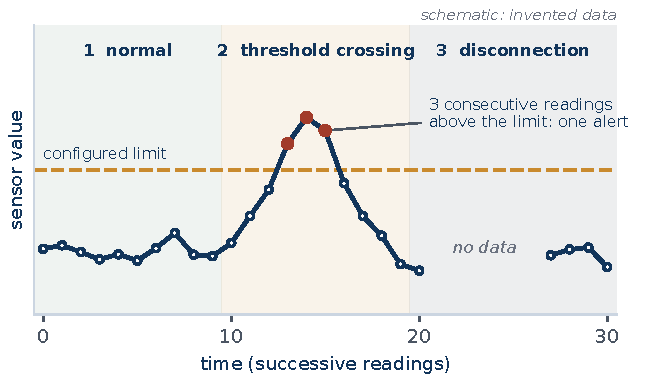
\includegraphics[width=7.3cm]{images/class28_evidence_stream.pdf}};
\foreach \y/\n/\ico/\col/\ttl/\txt in {0/1/check-circle/coursegreen/Normal behavior/{\texttt{nominal}: no alert; show connection, batch, and state.}, -1.4/2/exclamation-triangle/coursegold/Threshold crossing/{\texttt{hold\_undershoot}: below 71.0\,°C in Hold, one critical alert.}, -2.8/3/unlink/coursered/Disconnection/{Cut the network (not in the figure): show the screen and the record.}} {
  \node[tile, fill=white, draw=\col, very thick, anchor=north west, minimum width=5.8cm, minimum height=1.3cm] at (7.6,\y) {};
  \node[circle, fill=\col, text=white, minimum size=0.55cm, inner sep=0, font=\small\bfseries] at (8.0,\y-0.65) {\n};
  \node[anchor=west, font=\footnotesize\bfseries, text=courseblue] at (8.45,\y-0.22) {\faIcon{\ico}\ \ttl};
  \node[anchor=north west, text width=4.7cm, align=left, font=\scriptsize, inner sep=0pt] at (8.45,\y-0.45) {\txt};
}
\keyidea{-4.65}{Collect the evidence as you go: a log line, a screenshot, and a test identifier for every claim you make.}
\end{tikzpicture}
\coursefooter
\end{cframe}

\begin{cframe}{One traceability path}{\cterm{Traceability matrix}{a table linking each requirement to its acceptance criterion, implementation, and test.}}
\centering
\begin{tikzpicture}
\foreach \x/\w/\lab in {0/1.0/ID, 1.16/2.5/REQUIREMENT, 3.82/3.2/ACCEPTANCE CRITERION, 7.18/2.4/IMPLEMENTATION, 9.74/2.3/TEST EVIDENCE, 12.2/1.2/STATUS} {
  \node[chip, anchor=north west, minimum width=\w cm, minimum height=0.4cm, font=\tiny\bfseries] at (\x,0) {\lab};
}
% the example row from the brief
\foreach \x/\w/\txt in {0/1.0/{{\bfseries FR-04}}, 1.16/2.5/{Operator configures a temperature rule}, 3.82/3.2/{A configured threshold is used for subsequent readings}, 7.18/2.4/{Alert rule form and evaluator}, 9.74/2.3/{TC-08 screenshot or log}} {
  \node[tile, fill=white, draw=coursegreen!70, thick, anchor=north west, minimum width=\w cm, minimum height=1.0cm, text width={(\w-0.25)*1cm}, align=left, font=\scriptsize, inner sep=3pt] at (\x,-0.5) {\txt};
}
\node[tilegreen, anchor=north west, minimum width=1.2cm, minimum height=1.0cm, font=\scriptsize\bfseries, text=coursegreen] at (12.2,-0.5) {\faIcon{check}\ Passed};
\draw[arrowgold, line width=1.6pt] (1.0,-1.0) -- (1.16,-1.0);
\draw[arrowgold, line width=1.6pt] (3.66,-1.0) -- (3.82,-1.0);
\draw[arrowgold, line width=1.6pt] (7.02,-1.0) -- (7.18,-1.0);
\draw[arrowgold, line width=1.6pt] (9.58,-1.0) -- (9.74,-1.0);
\draw[arrowgold, line width=1.6pt] (12.04,-1.0) -- (12.2,-1.0);
% placeholders for the other rows
\foreach \y/\id in {-1.65/FR-05, -2.8/NFR-01} {
  \foreach \x/\w in {0/1.0, 1.16/2.5, 3.82/3.2, 7.18/2.4, 9.74/2.3, 12.2/1.2} {
    \node[tilegray, anchor=north west, minimum width=\w cm, minimum height=0.9cm] at (\x,\y) {};
  }
  \node[font=\tiny\bfseries, text=coursegray!70] at (0.5,\y-0.45) {\id};
}
\node[font=\tiny\itshape, text=coursegray] at (6.7,-3.82) {one row per requirement, filled in as the work progresses};
\keyidea{-4.1}{A traceability matrix answers two questions: why does this code exist, and how do we know it works? Follow one row from left to right.}
\end{tikzpicture}
\coursefooter
\end{cframe}

% ================================================================== PART 3
\sectiondivider{3}{Evolve and close}{sync-alt}{validation shows where the product stands; a change request tests how well the work can evolve.}{$\bullet$\ The change request and its impact\\[3pt]$\bullet$\ Retrospective: how the team worked}

\begin{cframe}{The change request}{\cterm{Release notes}{a short account of what changed in a release.}\cterm{SRS v2}{the specification after the change request has been analyzed and applied.}}
\centering
\begin{tikzpicture}
\node[chip, fill=coursegold, anchor=north west, minimum width=6.2cm, minimum height=0.55cm, font=\scriptsize\bfseries, align=left] at (0,0) {\faIcon{envelope-open-text}\ CHANGE REQUEST \ from Quality Management};
\node[tile, fill=white, draw=coursegold, thick, anchor=north west, minimum width=6.2cm, minimum height=1.95cm, text width=5.8cm, align=left, font=\footnotesize] at (0,-0.6) {During {\bfseries Hold}, temperature violations become critical only after a configurable number of consecutive readings. The recorded alert must include the process state in which it was raised.};
\foreach \y/\n/\t in {-2.8/1/Analyze the impact, -3.5/2/Update SRS v1 to v2 and the backlog, -4.2/3/Implement or plan the evolved increment} {
  \node[chip, fill=courseblue, anchor=north west, minimum width=6.2cm, minimum height=0.45cm, font=\scriptsize\bfseries, align=left] at (0,\y) {\n\ \ \t};
}
\draw[arrowgray] (3.1,-3.28) -- (3.1,-3.48);
\draw[arrowgray] (3.1,-3.98) -- (3.1,-4.18);
\node[anchor=west, font=\tiny\bfseries, text=coursegray] at (6.75,0.15) {ANALYZE ITS IMPACT ON};
\foreach \a in {90,30,-30,-90,-150,150} {
  \draw[courseblue!25, line width=1.5pt] (9.9,-2.15) -- ({9.9+2.35*cos(\a)},{-2.15+1.85*sin(\a)});
}
\node[circle, fill=coursegold, text=white, minimum size=1.3cm, inner sep=0, font=\scriptsize\bfseries, draw=white, line width=2pt, align=center] at (9.9,-2.15) {{\Large\faIcon{exchange-alt}}\\Change};
\foreach \a/\ico/\lab in {90/list-ol/Backlog, 30/file-alt/SRS, -30/vial/Tests, -90/cubes/Architecture, -150/desktop/Interface, 150/book/Operational guide} {
  \node[tile, fill=white, draw=coursegold!80, thick, minimum width=2.6cm, minimum height=0.5cm, font=\scriptsize, text=courseblue, inner sep=3pt] at ({9.9+2.35*cos(\a)},{-2.15+1.85*sin(\a)}) {\faIcon{\ico}\ \lab};
}
\end{tikzpicture}
\coursefooter
\end{cframe}

\begin{cframe}{Retrospective}{\cterm{Retrospective}{a short meeting where a team reviews how it worked and agrees what to change.}\cterm{Action}{one concrete change the team commits to try, with someone responsible.}}
\centering
\begin{tikzpicture}
\foreach \x/\col/\ico/\lab/\q/\sa/\sb/\ra/\rb in {0/coursegreen/thumbs-up/KEEP/{Which habit made your evidence easy to find and defend?}/stickygreen/stickyyellow/-2/1.5, 4.55/coursegold/sync-alt/CHANGE/{Where did an unclear question, an assumption, or a late change cost the most?}/stickyyellow/stickyblue/1.5/-1, 9.1/courseblue/lightbulb/TRY/{Which one practice from Class 25 will your team apply next time?}/stickyblue/stickygreen/-1/2} {
  \node[tile, fill=white, draw=\col, thick, anchor=north west, minimum width=4.3cm, minimum height=2.55cm] at (\x,0) {};
  \node[chip, fill=\col, anchor=north west, minimum width=3.9cm, minimum height=0.42cm, font=\tiny\bfseries, align=left] at (\x+0.2,-0.18) {\faIcon{\ico}\ \lab};
  \node[anchor=north west, text width=3.9cm, align=left, font=\scriptsize, inner sep=0pt] at (\x+0.2,-0.8) {\q};
  \sticky{\x+1.15}{-2.05}{\sa}{\ra}{}
  \sticky{\x+3.05}{-2.05}{\sb}{\rb}{}
}
\node[anchor=west, font=\tiny\bfseries, text=coursegray] at (0,-2.85) {HOW TO RUN IT, IN ABOUT TEN MINUTES};
\foreach \x/\n/\t in {0/1/Look back at both sessions, 4.55/2/Group the notes by theme, 9.1/3/Agree one change to try} {
  \node[chip, fill=courseblue, anchor=north west, minimum width=4.3cm, minimum height=0.5cm, font=\scriptsize\bfseries, align=left] at (\x,-3.05) {\n\ \ \t};
}
\draw[arrowgray] (4.3,-3.3) -- (4.55,-3.3);
\draw[arrowgray] (8.85,-3.3) -- (9.1,-3.3);
\keyidea{-3.85}{A retrospective is about the process, not about people. Leave with one concrete change the team will really try.}
\end{tikzpicture}
\coursefooter
\end{cframe}

% ------------------------------------------------------------------ closing
\section{Wrap-up}\gdef\currentsectionname{Wrap-up}
\begin{frame}{From this class to the next}
\centering
\begin{tikzpicture}
\foreach \i/\lab/\bg/\fg in {1/SE and ML/courseice/coursegray, 2/Requirements/courseice/coursegray, 3/Process/courseice/coursegray, 4/Design/courseice/coursegray, 5/Quality/courseblue/white, 6/Evolution/courseblue/white} {
  \node[rounded corners=3pt, minimum width=2.18cm, minimum height=0.6cm, font=\scriptsize\bfseries, fill=\bg, text=\fg] at ({1.1+(\i-1)*2.28},0) {\i\ \lab};
}
\node[font=\tiny\bfseries, text=courseblue] at (6.8,-0.52) {THIS CLASS PUTS QUALITY AND EVOLUTION TO WORK, ON THE REQUIREMENTS AND PROCESS OF CLASS 26};
\foreach \x/\sty/\ico/\ttl/\txt in {0/tileblue/lightbulb/What stays with us/{$\bullet$\ Validation is evidence, not opinion.\\[3pt]$\bullet$\ A change touches backlog, SRS, tests, and code.\\[3pt]$\bullet$\ Version 2 keeps the chain coherent.}, 4.55/tileblue/project-diagram/Use it in your project/{$\bullet$\ Keep a log line, a screenshot, and a test identifier for every claim.\\[3pt]$\bullet$\ Treat each change as an impact analysis, not as a patch.}, 9.1/tilegold/arrow-right/Next: Class 29/{\textbf{Online Learning and Concept Drift.}\\[3pt]The live stream returns in the next class: models that learn from each reading and the change they must detect.}} {
  \node[\sty, anchor=north west, minimum width=4.3cm, minimum height=3.8cm] at (\x,-0.95) {};
  \badge{\x+0.65}{-1.6}{courseblue}{\ico}
  \node[anchor=west, text width=3.0cm, align=left, font=\small\bfseries, text=courseblue] at (\x+1.2,-1.6) {\ttl};
  \node[anchor=north west, text width=3.9cm, align=left, font=\scriptsize] at (\x+0.2,-2.25) {\txt};
}
\node[tilegold, fill=white, anchor=north west, minimum width=13.4cm, minimum height=0.95cm, text width=12.6cm, align=left, font=\footnotesize] at (0,-5.0) {{\bfseries\goldink\faIcon{route}\ Course thread.} The strongest prototype is the one whose behavior can be explained and defended from stakeholder need to validation evidence.};
\end{tikzpicture}
\coursefooter
\end{frame}

\end{document}
